\documentclass[12pt]{article}
\usepackage[margin=1.0in]{geometry}
\usepackage{parskip}
\usepackage{graphicx}
\usepackage{caption}

\graphicspath{ {./images/} }


\begin{document}
\section*{Main DSP Concepts}

We can model an analog signal as a continuous function of time $x(t)$. We can model a digital signal as a discrete sequence $\{x_n\} = \cdots, x_{-2}, x_{-1}, x_0, x_1, x_2, \cdots$, essentially a list of numbers.  With a sampling period $t_s$, we can sample an analog signal $x(n)$ to generate a digital signal $\{x_n\}$ as follows: $\{x_n\} = x(nt_s)$, or equivalently with sampling period  $f_s$, $\{x_n\} = x(\frac{n}{f_s})$

We can define discrete systems that modify a discrete sequence, and write $\{y_n\} = T\{x_n\}$ for this, where $T$ is a discrete system. We can ascribe certain properties to discrete systems; most importantly linearity and time-invariance.

If a system $T$ is linear, then it holds that $T\{x_n + y_n\} = T\{x_n\} + T\{y_n\}$

If a system $T$ is time-invariant if it holds that for any $d$, $\{y_{n-d}\} = T\{x_{n-d}\}$

Systems that have both of these properties are referred to as linear time-invariant (LTI) systems, and are of particular importance because of certain properties about them that hold. For example, the impulse response of an LTI system completely characterizes it, by convolving the an input sequence with the system's impulse response.

\subsection*{The Fourier Transform}

An important operation in DSP is the Fourier transform, defined as follows on a continuous signal $x(t)$:

\[
  X(f) = \mathcal{F}\{x(t)\}(f) = \int_{-\infty}^\infty x(t)e^{-j 2 \pi f t} \mathrm{d}t
.\] 

Expanding $e^{-j2\pi f t}$, this can be rewritten as follows:
\[
  X(f) = \mathcal{F}\{x(t)\}(f) =  \int_{-\infty}^\infty x(t)\left[\cos(2\pi f t) - j\sin(2\pi f t)\right] \mathrm{d}t
.\] 

This makes the Fourier transform's purpose more obvious: we are decomposing a time signal into the frequencies of sine and cosine waves that make it up. Figure 1 shows the box function and its Fourier transform.

\begin{minipage}{\textwidth}
  \centering
  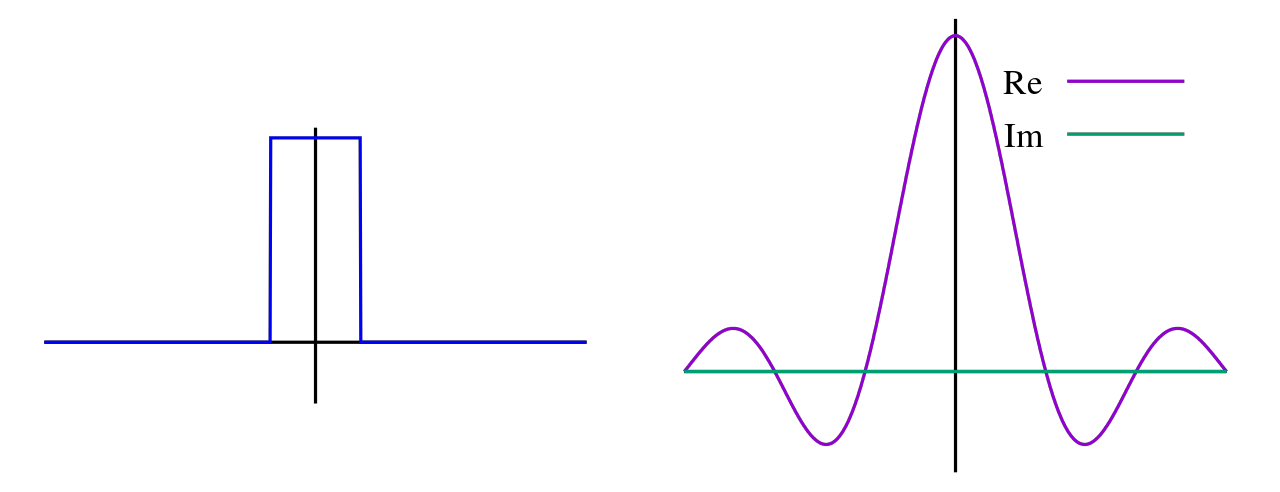
\includegraphics[trip=0 0 0, clip, scale=0.2]{fourier_transform}
  \captionof{figure}{Fourier transform of square wave}
\end{minipage}

The Fourier transform produces both real and imaginary components. If we only consider real signals, the real portion of the Fourier transform corresponds to the even parts of the signal (the cosine components), and the imaginary portion of the Fourier transform corresponds to the odd parts of the signal (the sine components). This means that the box function in Figure 1 has an entirely real Fourier transform, because it is an even function. Another property of the Fourier transform of real functions is that the the real and imaginary components will be even, so we do not gain any information from the negative parts of the transform.






\end{document}
